\section{Validazione}\label{validazione}

Illustreremo e commenteremo adesso le performance testando BlueAgent.
Per tutti i test e' stato eseguito BlueAgent all'interno di una macchina
virtuale con a disposizione 8 Core Ryzen 7700X, 16GB RAM 5600MHz e la
pool ZFS all'interno di un SSD.

I test effettuati si occupano di richiedere e misurare il tempo
richiesto per le seguenti fasi:

\begin{itemize}
\tightlist
\item
  B1: Provisioning per \(M\) team.
\item
  B2: Deploy di \(C\) container per ogni team.
\item
  B3: Lancio della verifica per ogni team
\item
  B4: Teardown dell'ambiente di verifica
\item
  B5: Teardown delle macchine
\item
  B6: Teardown delle infrastrutture dei team.
\end{itemize}

Per assicursi sincronia nelle misurazioni, il test e' stato organizzato
in barriere \(B1,\dots,B6\). Per superare una barriera si attende che
tutte le operazioni sulle risorse siano completate, cosi da vitare
misurazioni errate.

Ad ogni banda vengono eseguite una serie di richieste HTTP verso
BlueAgent mentre ogni 100ms si campiona il contenuto di
\passthrough{\lstinline!/proc/stat!} per ottenere:

\begin{itemize}
\tightlist
\item
  \(\text{CPU}_{\text{util}} = \Delta (\text{user} + \text{system} + \text{nice}) / \Delta \text{total} \times 100\)
\item
  \(\text{IO}_{\text{wait}} = \Delta \text{iowait} / \Delta \text{total} \times 100\)
\end{itemize}

\begin{quote}
spiega che vordi sta roba
\end{quote}

Per ottenere l'uso della RAM invece sono stati campionati
\passthrough{\lstinline!/proc/meminfo!} e
\passthrough{\lstinline!/proc/spl/kstat/zfs/arcstats!} per ottenere:

\begin{itemize}
\tightlist
\item
  \(\text{RAM}_{\text{usata\_grezza}} = \text{MemTotal} - \text{MemFree} - \text{Buffers} - \text{Cached}\)
\item
  \(\text{RAM}_{\text{netta\_container}} = \text{RAM}_{\text{usata\_grezza}} - \text{ARC}_{\text{size}} - \text{RAM}_{\text{baseline}}\)
\end{itemize}

\begin{quote}
spiega che vordi sta roba
\end{quote}


\begin{figure}[htbp]
  \centering
  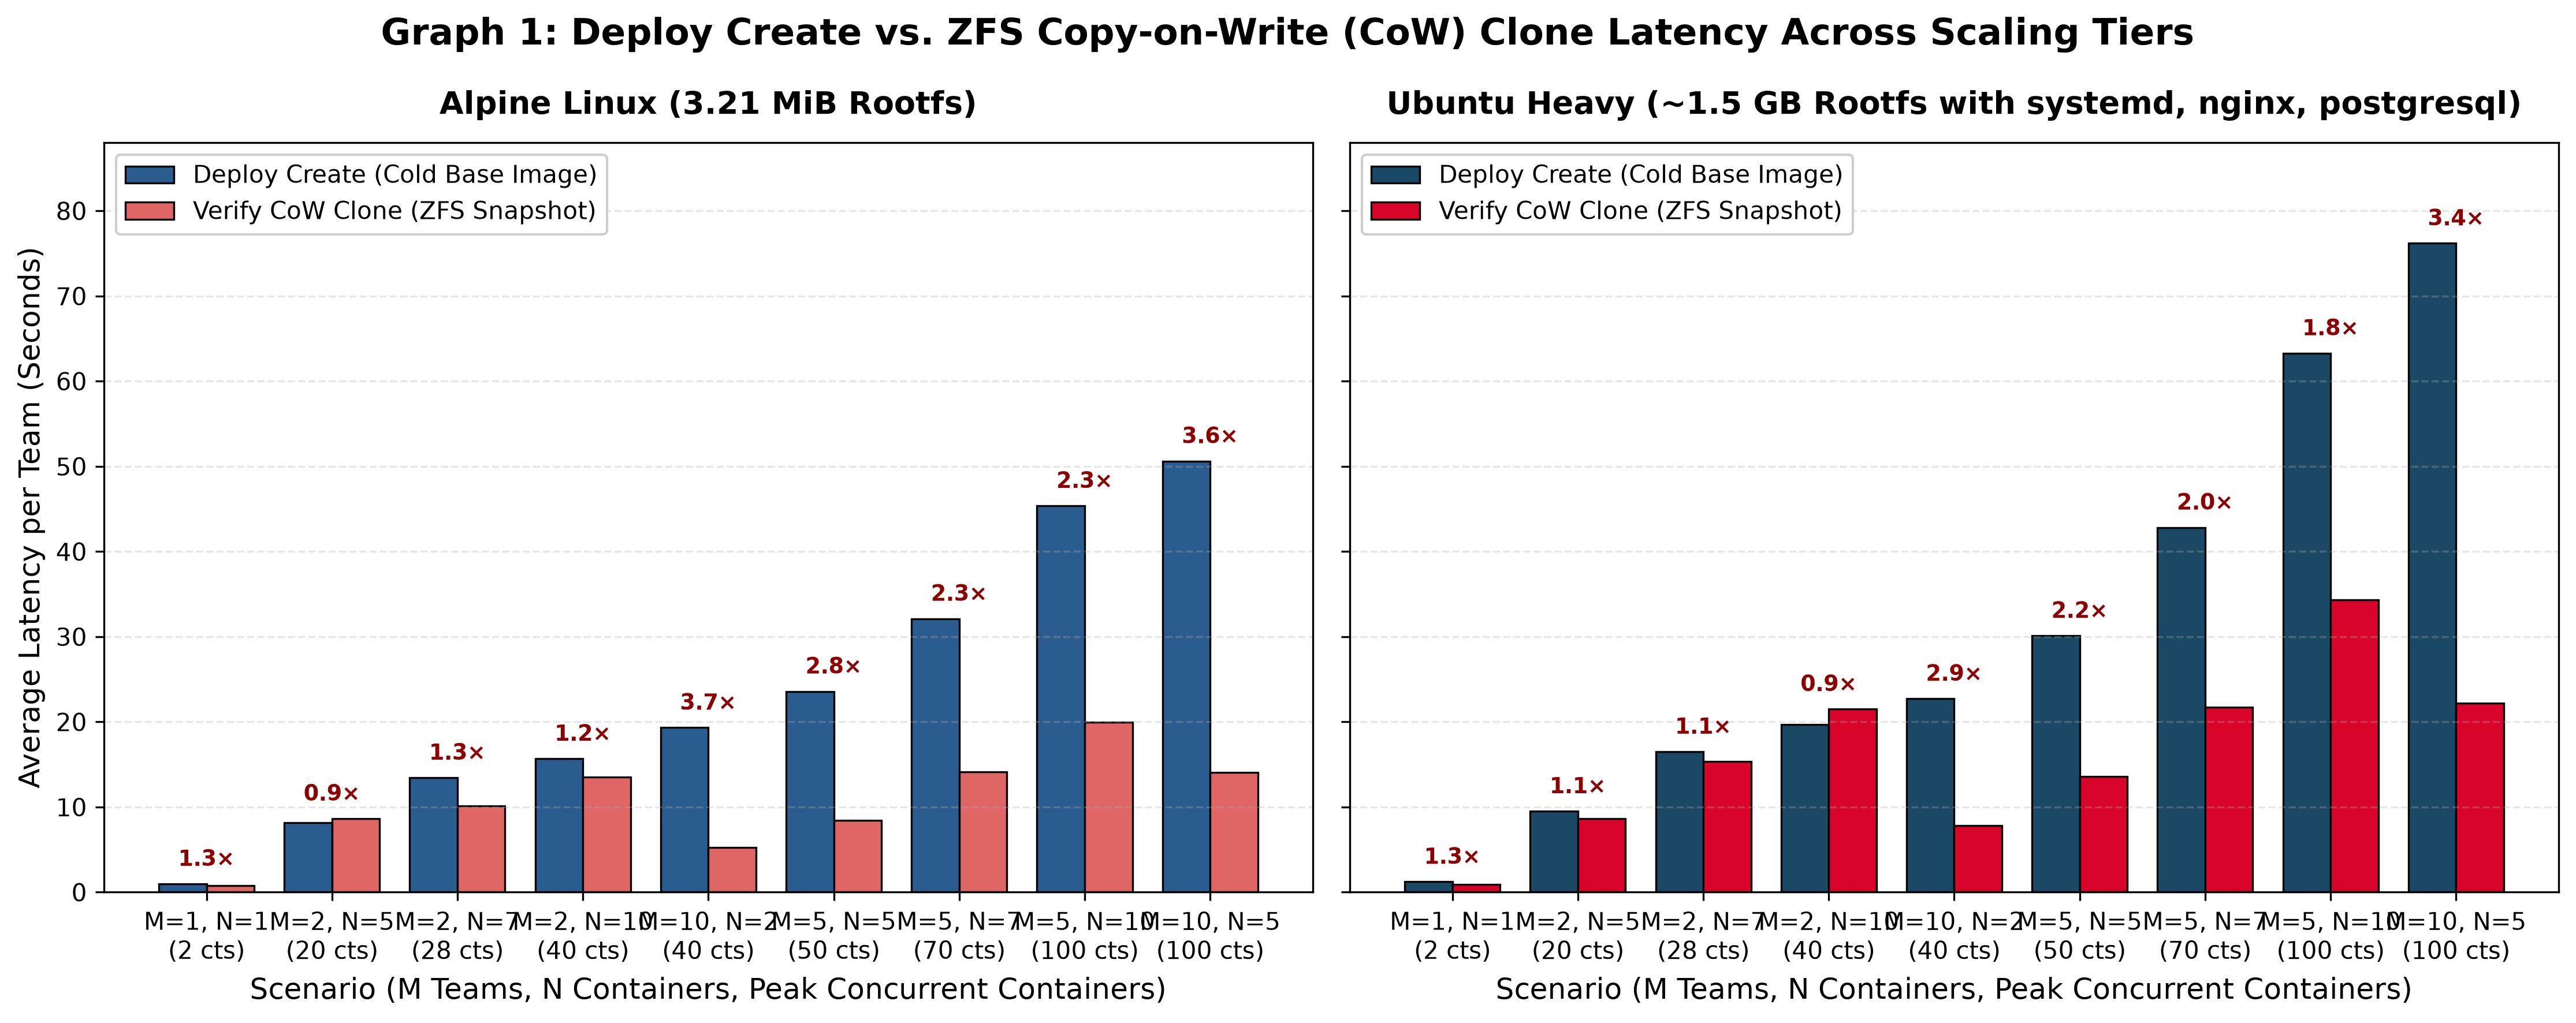
\includegraphics[width=0.92\linewidth,height=0.7\textheight,keepaspectratio]{src/images/graph1_cow_vs_deploy.png}
  \caption{Graph1 Cow Vs Deploy}
  \label{fig:graph1_cow_vs_deploy}
\end{figure}



\begin{figure}[htbp]
  \centering
  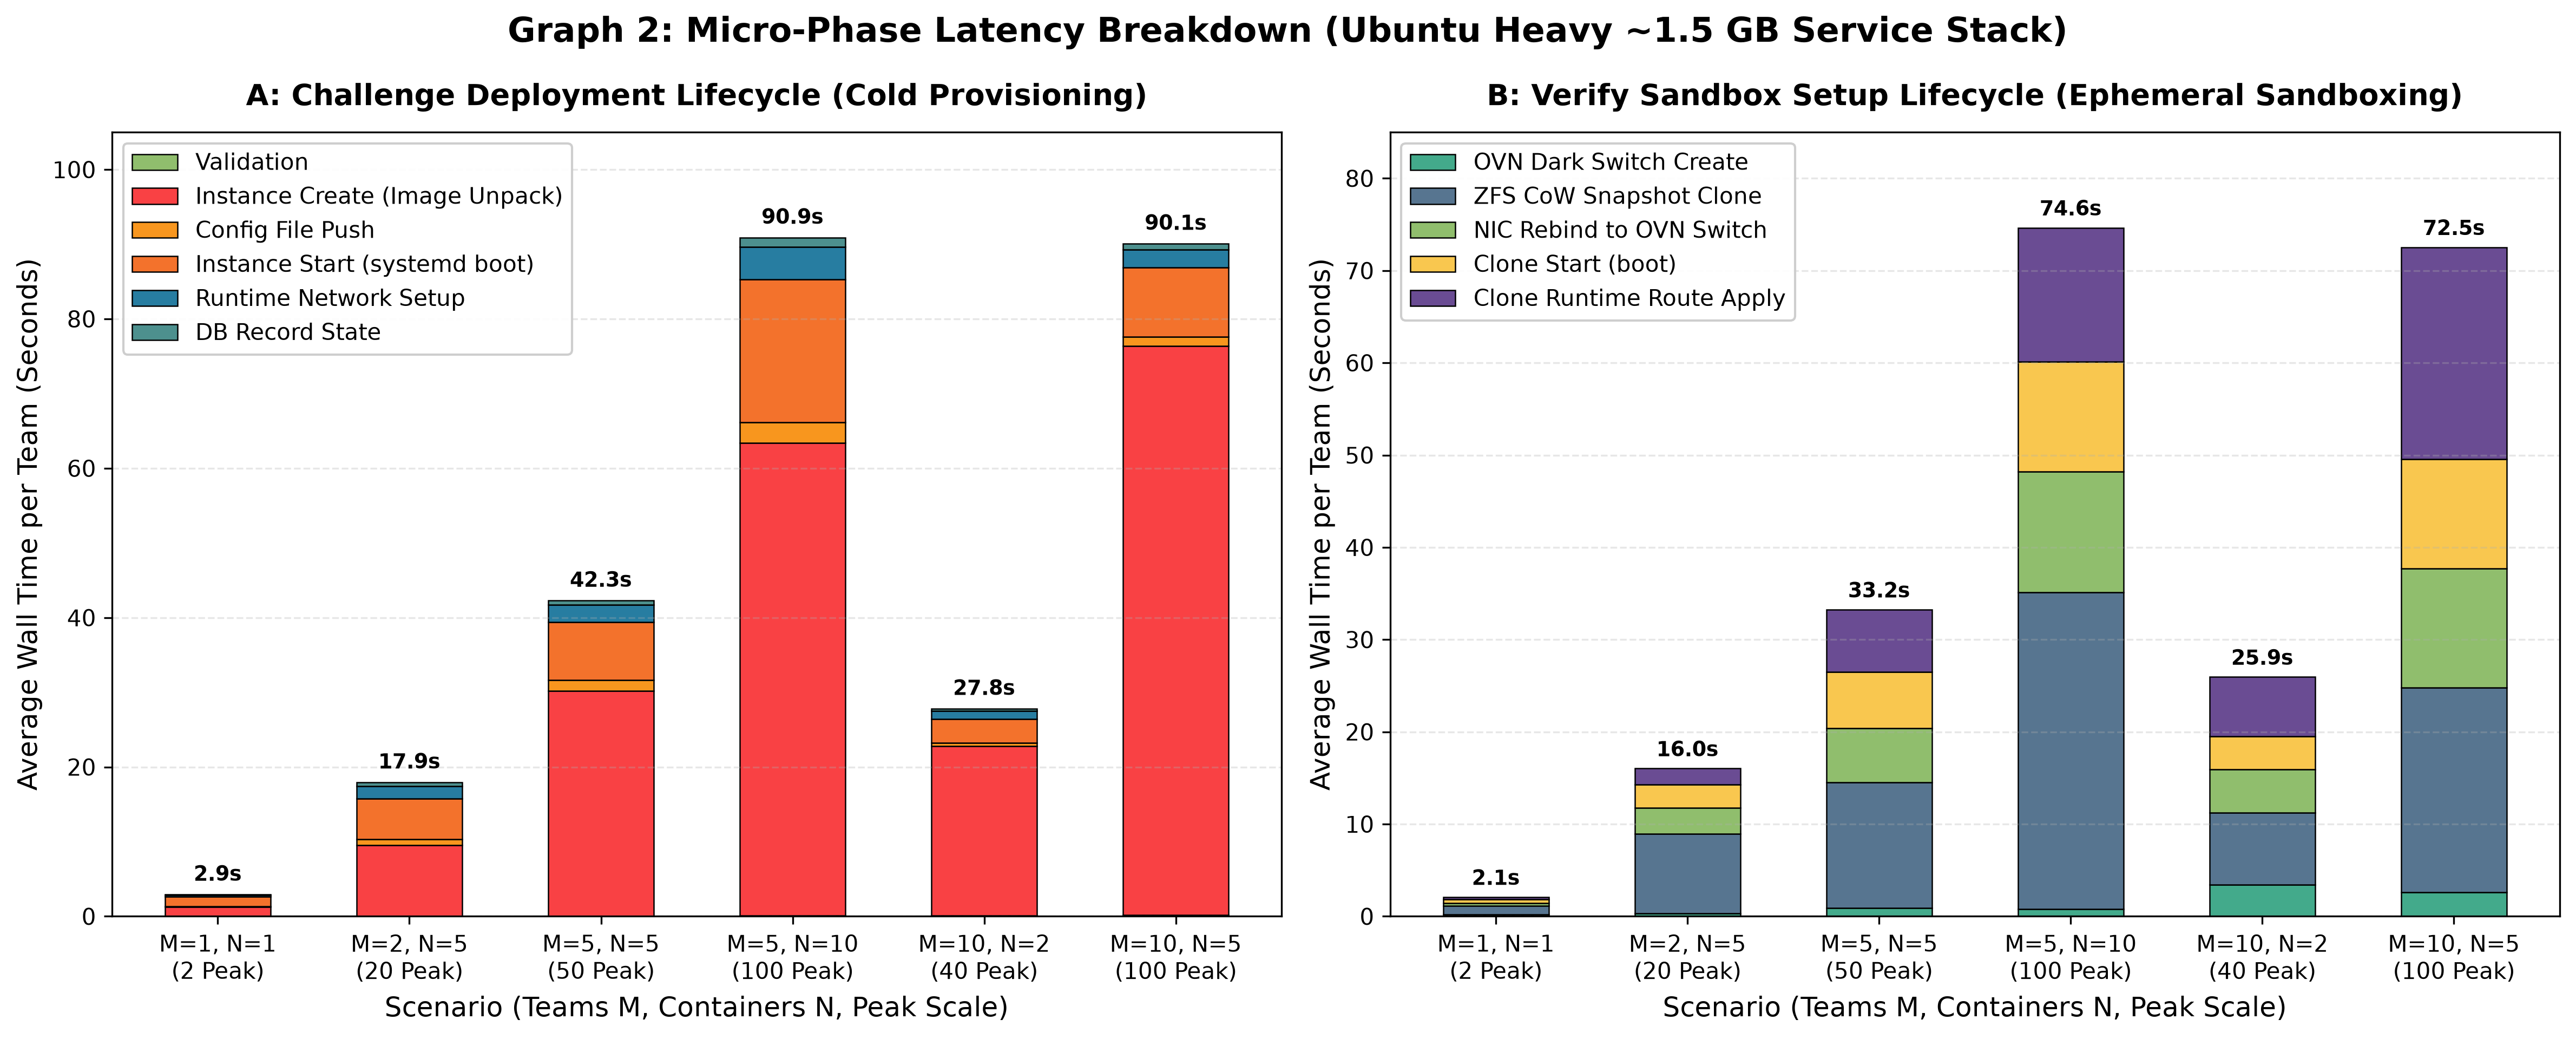
\includegraphics[width=0.92\linewidth,height=0.7\textheight,keepaspectratio]{src/images/graph2_microphase_breakdown.png}
  \caption{Graph2 Microphase Breakdown}
  \label{fig:graph2_microphase_breakdown}
\end{figure}



\begin{figure}[htbp]
  \centering
  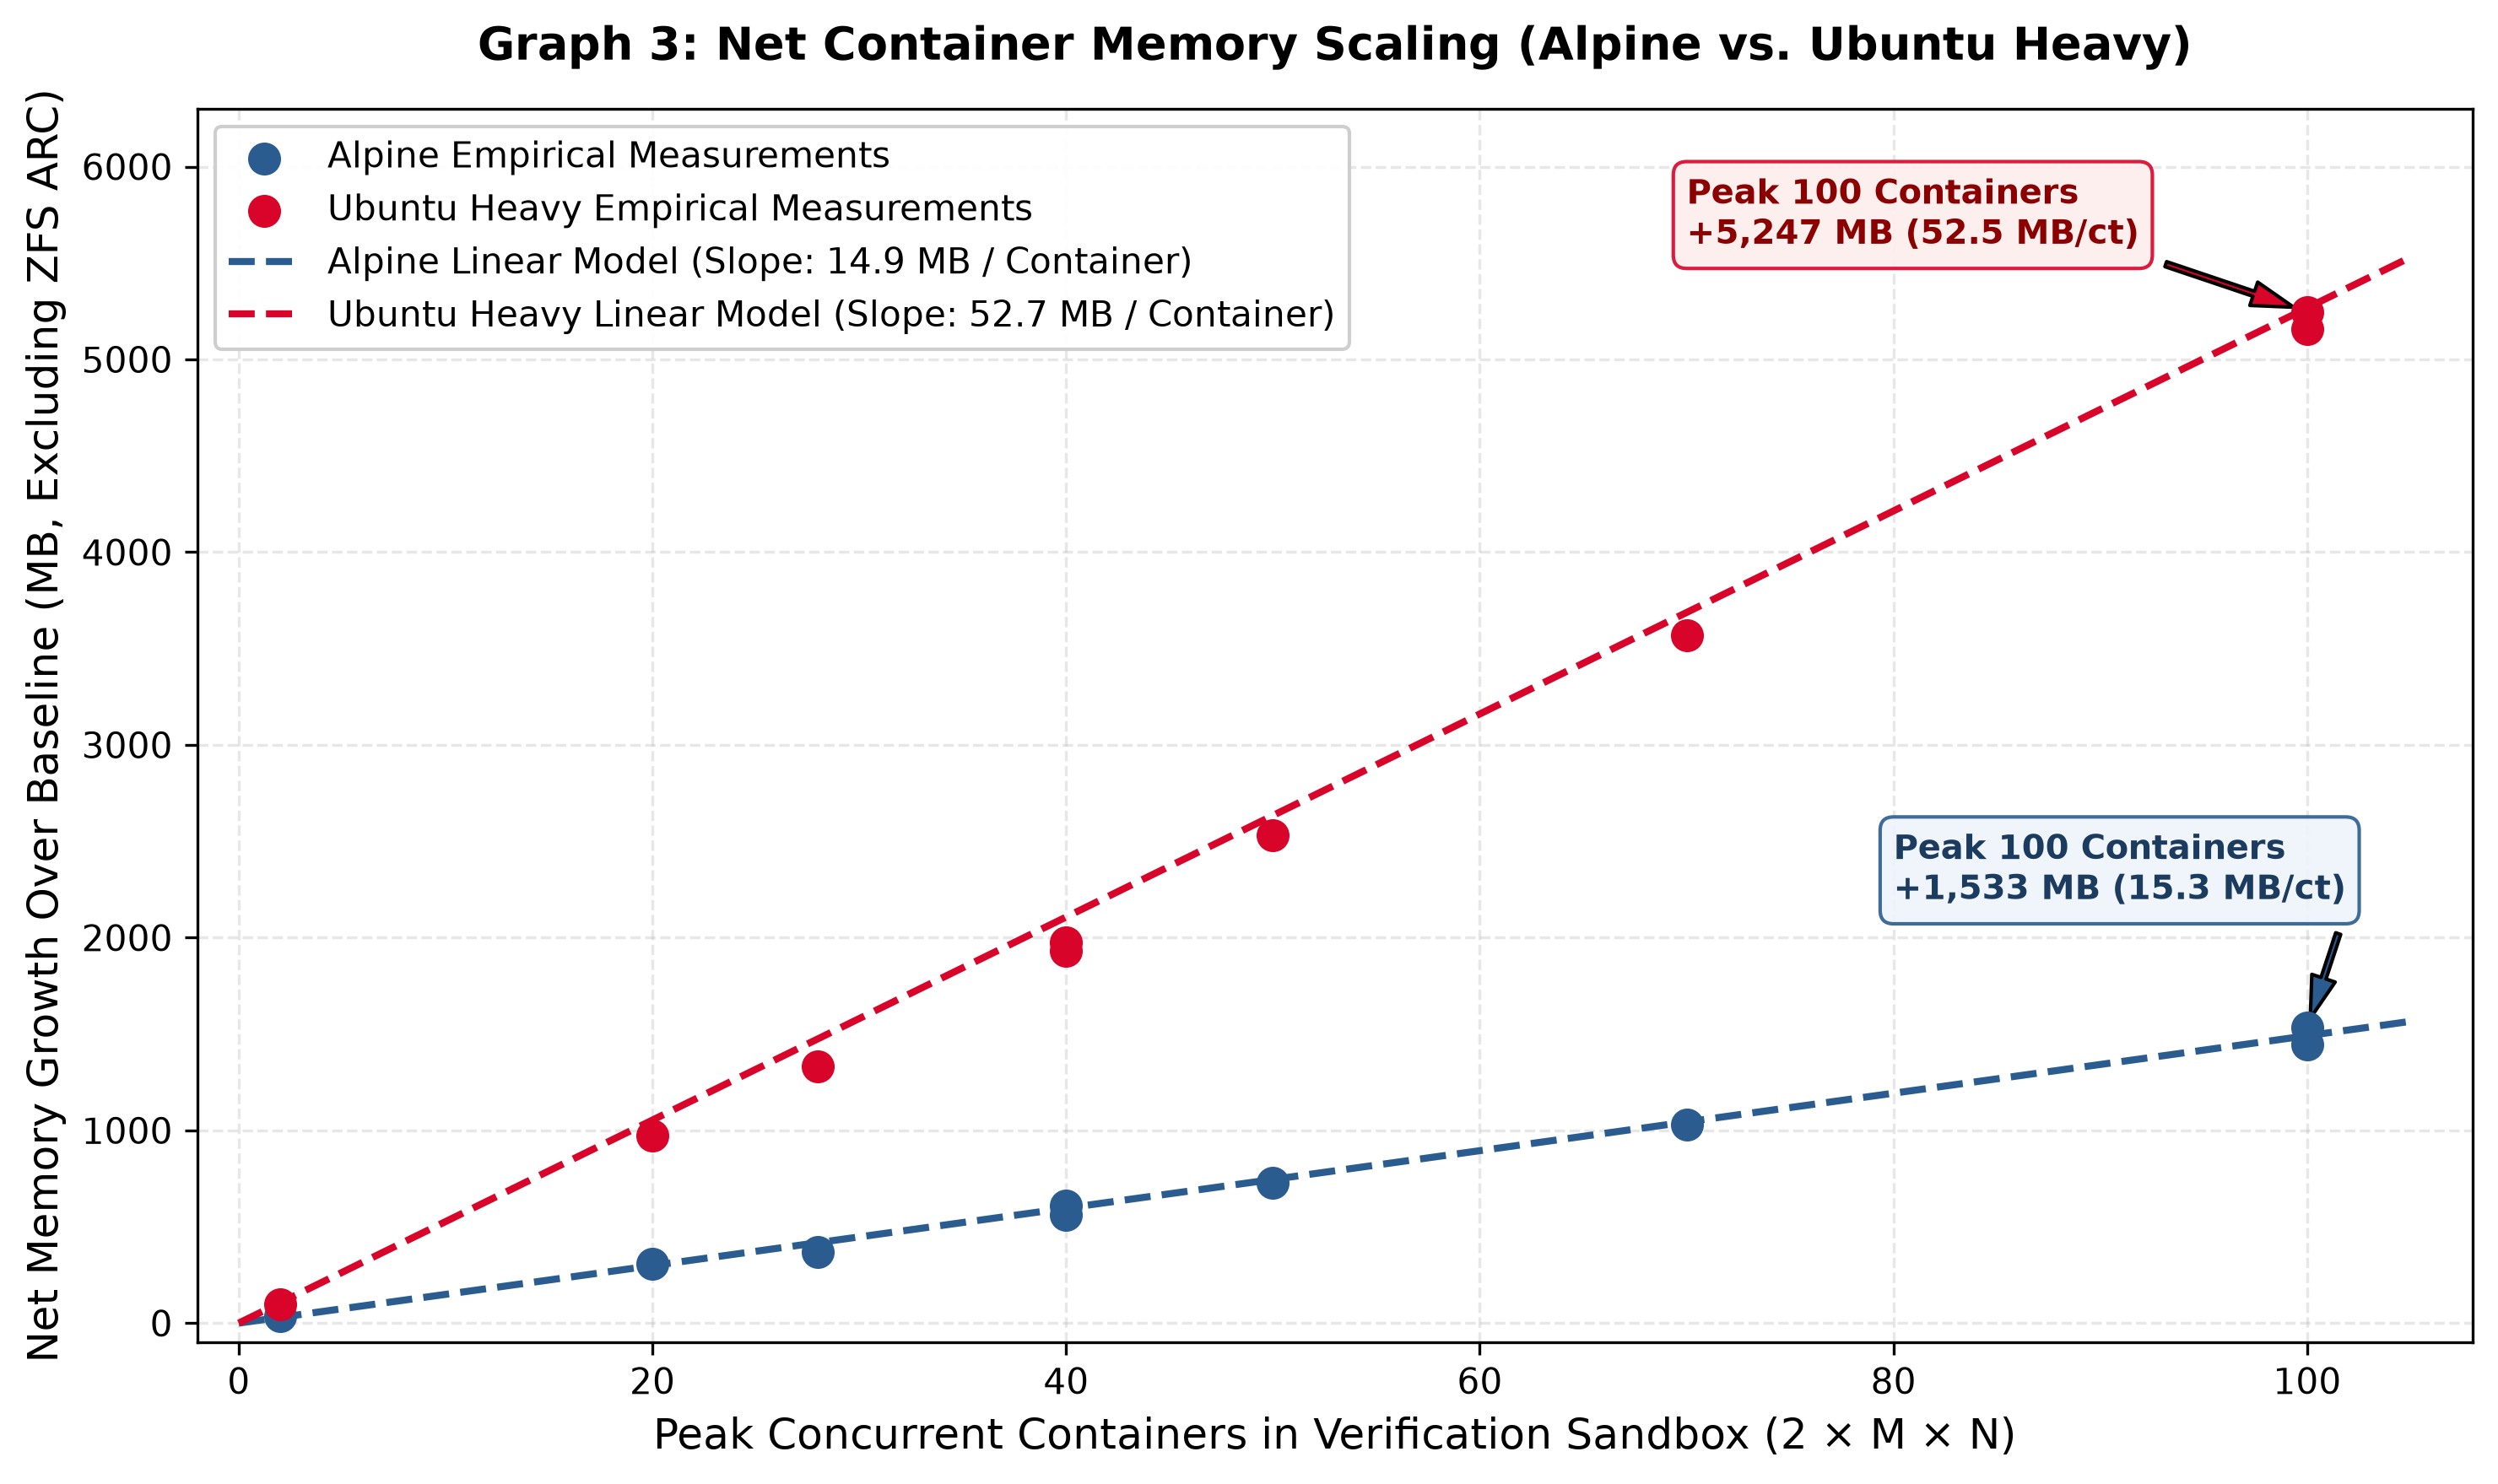
\includegraphics[width=0.92\linewidth,height=0.7\textheight,keepaspectratio]{src/images/graph3_memory_scaling.png}
  \caption{Graph3 Memory Scaling}
  \label{fig:graph3_memory_scaling}
\end{figure}

